\documentclass[main.tex]{subfiles}
 
\begin{document}

\chapterimage{band1.jpg}
\chapter{Network Configuration}

In this step we will build a firmware such that the end-user can configure her Wi-Fi network's credentials into the device at run-time. Since a user's network credentials will be stored persistently on the device, we will also provide a \textit{Reset to Factory} action where a user's configurations can be erased from the device.
You may refer to the \textit{4\_network\_config/} directory of esp-jumpstart for looking at this code.

In the previous example, we had hard-coded the Wi-Fi credentials into the firmware. This obviously doesn't work for a end-user product.

\section{Overview}\index{Overview}
As can be seen in this figure, in the network configuration stage, the end-user typically uses her smart-phone to \textit{securely} configure her Wi-Fi credentials into your device. Once the devices acquires these credentials, it can then connect to her home Wi-Fi network. 

\begin{figure}
    \centering
    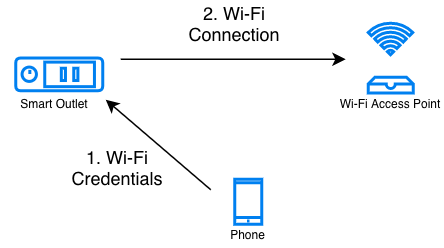
\includegraphics[scale=0.4]{../../_static/network_config.png}
    \caption{Network Configuration Process}
    \label{fig:network_config}
\end{figure}

There can be multiple channels through which your device can receive the Wi-Fi credentials. ESP32 supports the following mechanisms:

\begin{itemize}
    \item SoftAP 
    \item Bluetooth Low Energy (BLE)
    \item Smart-Config
\end{itemize}

Each of these have their own pros and cons. There is no single correct way of doing this, some developers may pick one way, and some the other, depending upon what you value more.

\subsection{SoftAP}\index{SoftAP}
In the SoftAP mechanism your outlet will launch its own temporary Wi-Fi Access Point. The user can then connect their smart-phones to this temporary Wi-Fi network. And then use this connection to transfer the Home Wi-Fi's credentials to the outlet. Many connected devices in the market today use this kind of mechanism. In this network configuration workflow, the user has to 
\begin{itemize}
    \item switch their phone's Wi-Fi network to your outlet's temporary Wi-Fi network
    \item launch your phone application
    \item enter her home Wi-Fi credentials that will be then transferred to the outlet over the SoftAP connection
\end{itemize}
From a user experience perspective, the first step of this requires the user to change their phone's Wi-Fi network. This may be confusing to some users. Additionally, changing the Wi-Fi network programatically through the phone application may not always be possible (iOS and some variants of Android don't allow application to this). The advantage of this method though is that it is very reliable (SoftAP being just Wi-Fi is an established mechanism), and doesn't require a lot of additional code (since it's all over Wi-Fi).

\subsection{BLE}\index{BLE}

In the Bluetooth Low Energy (BLE) method, your outlet will be doing a BLE advertisement. Phones in the vicinity can see this advertisement, and ask the user to do a BLE connection with your device. Then this network is used to transfer the credentials to the outlet.
In this network configuration workflow, the user doesn't have to do the hard task of switching between Wi-Fi networks. Additionally, both iOS and Android allow phone application to scan for BLE devices in the vicinity and also connect to them through the app. This means a much smoother end-user experience.

One side-effect, though, of using the BLE based network configuration is that it also pulls in the code for Bluetooth. This means your flash requirement may be affected since your firmware size will increase. During the network configuration mode, BLE will also consume memory until the network configuration is complete.

\subsection{Smart-Config}\index{Smart-Config}
XXX

\section{Demo}\index{Demo}
Before getting into the details of the network configuration workflow, let us get a feel for how an end-user will configure the network using the provided application.
You may refer to the \textit{4\_network\_config/} directory of esp-jumpstart for trying this out.

\begin{itemize}
    \item Go to the \textit{4\_network\_config} application.
    \item Build, flash and load the application.
    \item By default, the firmware is launched in BLE mode.
    \item Install the companion phone application for network configuration from this location: \url{https://github.com/espressif/esp-idf-provisioning-android/releases}. Please install the latest app with \textbf{sec1-ble} as part of its name.
    \item Launch the application and follow the wizard as shown in the images below.
\end{itemize}

\ksnotebox{As of now, only Android users can try the application out. For iOS users, we are working on enabling an application with \textit{TestFlight} soon.}

XXX add network configuration images

\begin{itemize}
    \item If all goes well, your device would be connected to your Home Wi-Fi network.
    \item If you now reset the device, it will not enter the network-configuration mode. Instead it will go and connect to the Wi-Fi network that is configured.
\end{itemize}

 
\section{Unified Provisioning}\index{Unified Provisioning}\label{sec:unified_prov}

Espressif provides a \textbf{Unified Provisioning} module for assisting you with your network configuration. When this module is invoked from your firmware executable, the module takes care of managing all the state transitions (like starting/stopping the softAP/BLE interface, exchanging the credentials securely, storing them for subsequent use etc).

\begin{itemize}

\item Extensible Protocol: The protocol is completely flexible and it offers the ability for the developers to send custom configuration in the provisioning process. The data representation too is left to the application to decide.
\item Transport Flexibility: The protocol can work on Wi-Fi (SoftAP + HTTP server) or on BLE as a transport protocol. The framework provides an ability to add support for any other transport easily as long as command-response behaviour can be supported on the transport.
\item Security Scheme Flexibility: It’s understood that each use-case may require different security scheme to secure the data that is exchanged in the provisioning process. Some applications may work with SoftAP that’s WPA2 protected or BLE with “just-works” security. Or the applications may consider the transport to be insecure and may want application level security. The unified provisioning framework allows application to choose the security as deemed suitable.
\item Compact Data Representation: The protocol uses Google Protobufs as a data representation for session setup and Wi-Fi provisioning. They provide a compact data representation and ability to parse the data in multiple programming languages in native format. Please note that this data representation is not forced on application specific data and the developers may choose the representation of their choice.

\end{itemize}

\ksnotebox{More details about Unified provisioning are available at: \url{https://docs.espressif.com/projects/esp-idf/en/latest/api-reference/provisioning/provisioning.html}}

The following components are offered:
\begin{itemize}
    \item \textbf{Unified Provisioning Specification:} A specification to \textit{securely} transfer Wi-Fi credentials to the device, independent of the transport (SoftAP, BLE)
    \item \textbf{IDF Components:} Software modules that implement this specification in the device firmware, available through ESP-IDF
    \item \textbf{Phone Libraries:} Reference implementations on iOS and Android are available that can be directly incorporated into your existing phone applications
    \item \textbf{Reference Phone Applications:} Fully functional Phone applications on Android (\url{https://github.com/espressif/esp-idf-provisioning-android}) and iOS (\url{https://github.com/espressif/esp-idf-provisioning-ios}) are available for testing during your development, or for skinning with your brand's elements.
\end{itemize}

\subsection{The Code}\index{The Code}\label{sec:unified_prov}
The code for invoking the unified provisioning through your firmware is shown below:
\begin{minted}{c}

if (conn_mgr_prov_is_provisioned(&provisioned) != ESP_OK) {
    return;
}

if (provisioned != true) {
    /* Starting unified provisioning */
    conn_mgr_prov_start_provisioning(prov_type,
               security, pop, service_name, service_key);
} else {
    /* Start the station */
    wifi_init_sta();
}
\end{minted}

The \textit{conn\_mgr\_prov} component provides a wrapper over the unified provisioning interface. Some notes about the code above:
\begin{itemize}
    \item The \textit{conn\_mgr\_prov\_is\_provisionined()} API checks whether Wi-Fi network credentials have already been configured or not. These are typically stored in a flash partition called the \textit{NVS}. More about NVS later in this Chapter.
    \item If no Wi-Fi network credentials are available, the firmware launches the unified provisioning using the call \textit{conn\_mgr\_prov\_start\_provisioning()}. This API will take care of everything, specifically:
    \begin{enumerate}
        \item It will start the SoftAP or BLE transport as configured
        \item It will enable the necessary advertisements using the Wi-Fi or BLE standards
        \item It will \textit{securely} accept any network credentials from a phone application
        \item It will store these credentials, for future use, in the NVS
        \item Finally, it will deinitialise any components (SoftAP, BLE, HTTP Server etc) that were required by the unified provisioning mechanism. This ensures that this point onward there is almost no memory overhead from the unified provisioning module.
    \end{enumerate}
    \item If a Wi-Fi network configuration was found in NVS, we directly start the Wi-Fi station interface using \textit{wifi\_init\_sta()}.
\end{itemize}

These steps ensure that the firmware launches the unified provisioning module when no configuration is found, and if a configuration is available, then starts the Wi-Fi station interface.

Additionally, the unified provisioning module also needs to know the state transitions of the Wi-Fi interface. Hence an additional call needs to be made from the event handler for taking care of this:
\begin{minted}{c}
esp_err_t event_handler(void *ctx, system_event_t *event)
{
     conn_mgr_prov_event_handler(ctx, event);
   
     switch(event->event_id) {
     case SYSTEM_EVENT_STA_START:
...
...
...
\end{minted}

\subsubsection{Configurable Options}\index{Configurable Options}
In the code above, we have used the following call for invoking the unified provisioning interface:
\begin{minted}{c}
    /* Starting unified provisioning */
    conn_mgr_prov_start_provisioning(prov_type,
               security, pop, service_name, service_key);
\end{minted}

Let us now look at the parameters, or the configuration options of this API:
\begin{enumerate}
    \item \textbf{Transport:} The developer can choose which transport mechanism will be used for the network configuration. The options available are SoftAP or BLE. 
    \begin{itemize}
        \item The module is written in such a manner that, based on the developer's selection, only the relevant software libraries will get pulled into the final executable image. 
        \item The unified provisioning module will also manage the state transitions, and other services, that are required for the network configuration to take place
    \end{itemize}
    \item \textbf{Service Name:} When the user launches the network configuration app, the user will be presented with a list of unconfigured devices, in her vicinity. The service name is this name that will be visible to the user. You may choose a name that identifies your device conveniently (abc-thermostat). It is common practice to have some element in the service name that is unique or random. This helps in scenarios when there could be multiple unconfigured devices that the user is configuring at the same time.
    \item \textbf{Proof of Possession:} When a user brings in a new smart device, the device launches its provisioning network (BLE, SoftAP) for configuration.  How do you make sure that only the owner of the device configures the device and not their neighbours? This configurable option is for that. Please read the following subsection for more details about this option.
    \item \textbf{Security:} The unified provisioning module currently supports two security methods for transferring the credentials: \textit{security0} and \textit{security1}. Security0 uses no security for exchanging the credentials. This is primarily used for development purposes. Security1 uses elliptic curve, \textit{curve25519} crypto for key exchange, followed by \textit{AES-CTR} encryption for data exchanged on the channel.
\end{enumerate}

\subsubsection{Proof of Possession}\index{Proof of Possession}

When a user brings in a new smart device, the device launches its provisioning network (BLE, SoftAP) for configuration.  How do you make sure that only the owner of the device configures the device and not their neighbours?

Some products expect the user configuring the device to provide a proof that they really own (or posses) the device that they are configuring. The proof of possession can be provided by taking some physical action on the device, or by entering some unique random key that is pasted on the device's packaging box, or by displaying on a screen, if the device is equipped with one.

At manufacturing, every device can be programmed with a unique random key. This key could then be provided to the unified provisioning module as a proof of possession option. When the user configures the device using the phone application, the phone application transfers the proof of possession to the device. The unified provisioning module then validates that the proof of possession matches and then confirms the configuration.

\subsection{Additional Details}\index{Additional Details}

More details about Unified provisioning are available at: \url{https://docs.espressif.com/projects/esp-idf/en/latest/api-reference/provisioning/provisioning.html}

\section{NVS: Persistent key-value store}\index{NVS: Persistent key-value store}\label{sec:nvs_info}
In the Unified Provisioning section above, we mentioned in passing that the Wi-Fi credentials are stored in the NVS. The NVS is a software component that maintains a persistent storage of key-value pairs. Since the storage is persistent this information is available even across reboots and power shutdowns. The NVS uses a dedicated section of the flash to store this information.

The NVS is designed in such a manner so as to be resilient to metadata corruption across power loss events. It also takes care of wear-levelling of the flash by distributing the writes throughout the NVS partition.

Application developers can also use the NVS to store any additional data that you wish to maintain as part of your application firmware. Data types like integers, NULL-terminated strings and binary blobs can be stored in the NVS. This can be used to maintain any user configurations for your product. Simple APIs like the following can be used to read and write values to the NVS.

\begin{minted}{c}
  /* Store the 'chosen_value' variable to NVS */
  nvs_set_u32(nvs_handle, "my_key", chosen_value);

  /* Read the 'chosen_value' variable from NVS */
  nvs_get_u32(nvs_handle, "my_key", &chosen_value);
\end{minted}


\subsection{Additional Details}\index{Additional Details}

More details about NVS are available at: \url{https://docs.espressif.com/projects/esp-idf/en/latest/api-reference/storage/nvs_flash.html}

\section{Reset to Factory}\index{Reset to Factory}
Another common behaviour that is expected of products is \textit{Reset to Factory Settings}. Once the user configuration is stored into the NVS as discussed above, reset to factory behaviour can be achieved by simply erasing the NVS partition.

Generally, this action is triggered by long-pressing a button available on the product. This can easily be configured using the \textit{iot\_button\_*()} functions

\subsection{The Code}\index{The Code}\label{sec:reset_to_factory}
In the \textit{4\_network\_config/} application, we use a long-press action of the same toggle push-button to configure the reset to factory behaviour.

\begin{minted}{c}
/* Register 3 second press callback */  
iot_button_add_on_press_cb(btn_handle, 3, button_press_3sec_cb, NULL);
\end{minted}

This function makes the configuration such that the \textit{button\_press\_3sec\_cb()} function gets calls whenever the button associated with the \textit{btn\_handle} is pressed and released for longer than 3 seconds. Remember we had initialised the \textit{btn\_handle} in our Chapter \ref{the-outlet}

Then callback function can then be written as follows:
\begin{minted}{c}
static void button_press_3sec_cb(void *arg)
{
    nvs_flash_erase();
    esp_restart();
}
\end{minted}

This code basically erases all the contents of the NVS, and then triggers a restart. Since the NVS is now wiped, the next time the device boots-up it will go back into the unconfigured mode. 

If you have loaded and configured the device with the \textit{4\_network\_config/} application, you can see this in action and by pressing the toggle button for more than 3 seconds and then releasing it.

\section{Progress so far}\index{Progress so far}
Now we have a smart outlet that the user can configure, through a phone app, to their home Wi-Fi network. Once configured, the outlet will keep connecting to this configured network. We also have the ability to erase these settings on a long-press of a push-button.

As of now, the outlet functionality and the connectivity functionality are separate. As our next step, let's control and monitor the state of the outlet (on/off) remotely.
\end{document}
